\documentclass[11pt,a4paper]{article}

\usepackage{titling}
\usepackage[hidelinks]{hyperref}
\usepackage{graphicx}
\usepackage{grffile}
\usepackage{float}
\usepackage{geometry}

\newcommand{\subtitle}[1]{
  \posttitle{
    \par\end{center}
    \begin{center}\large#1\end{center}
    \vskip0.5em}
}

\begin{document}


\title{Hyper Perform\\ Functional Requirements Specification}
\subtitle{ Organisation: \url{https://github.com/Hyperperform}}
\begin{figure}
			\centering
			
\includegraphics[height=200px]{../Images/CodusMaximus_logo.jpg}
\end{figure}

	
\author{
	\textbf{Developers:} \\
	Claudio Da Silva	\emph{14205892}	\\
	Rohan Chhipa		\emph{14188377}	\\
	Avinash Singh		\emph{14043778}	\\
	Jason Gordon		\emph{14405025}	\\\\
}

\date{\textbf{Updated \today}}

\maketitle
\thispagestyle{empty}
\pagebreak

\tableofcontents
\pagebreak

\section{Introduction}
Many different tools are available for measuring the quality of products made, but very few tools exist which assess the quality of the people making said products. People play a huge role in a project, and trying to monitor each and every one becomes a tedious task which diverts man power away from other more critical tasks. Whether it be for an end of year evaluation, or attempting to assess the current status of a project, generating a report on a staff member can help keep up productivity, as well as get them any help they need in order to resume quality performance. By ensuring that there is constant quality performance from each individual on a project, one can increase project quality as well as reduce project risks such as loss of an important team member during a critical stage of a project's life-cycle. 

\section{Vision and Objectives}
\subsection{Vision}
The vision of this project is to create an automated performance management system, which can assess the performance and status of staff members, based on information sourced through various software systems such as card readers, version control systems and such. The system would make use of these external integrations as well as direct contact with the staff members via either web dashboard or mobile phone, to generate reports on the various staff members as well as add elements such as gamification and monitor problems that may be occurring.

\subsection{Objectives}
The objectives for the Hyper Perform system are:
\begin{itemize}
	\item To source information from various integrations and treat them as events to determine performance.
	\item To generate real-time reports on staff members in order to evaluate performance based on these events.
	\item To monitor staff members in order to determine possible causes of work detriment.
	\item To add a form of gamification to encourage productivity, and discourage slacking and other bad behaviours.
	\item To make the system easily expandable to various other sub-systems.
\end{itemize}



\section{User Management}
\subsection{Scope}
\begin{figure}[H]
	\begin{center}
		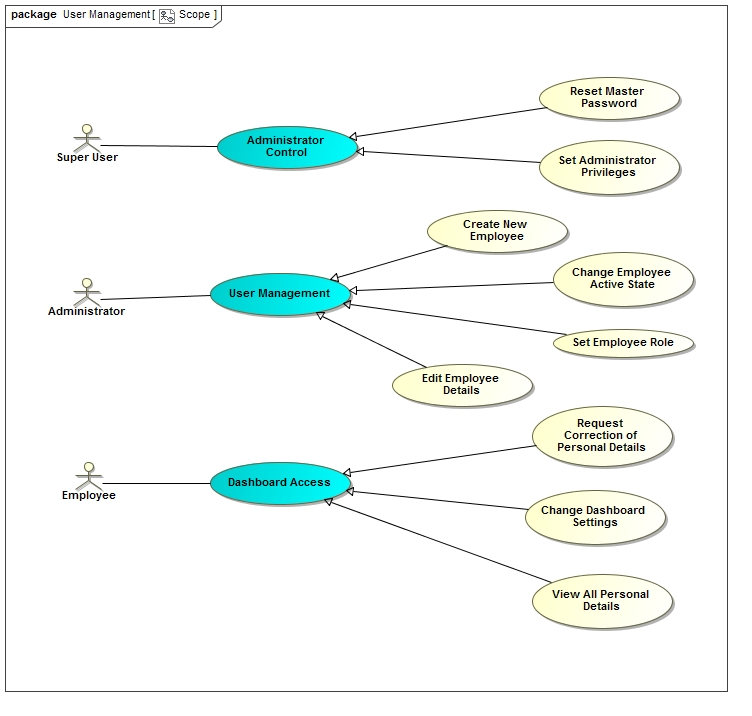
\includegraphics[scale=0.6]{../Images/User_Management_Scope.jpg}
		\caption{User Management Scope}
	\end{center}
\end{figure}

\pagebreak

The scope of the user management module includes:
\begin{itemize}
	\item Super user control over administrator rights given to individuals and only one super user can exist at any moment.
	\item Administrators may add employees and manage their details.
	\item Administrators may add employee roles to employees registered, which will define which algorithms and systems will influence their performance ratings.
	\item A user should be able to view all their personal details, and request change immediately if something is wrong. 
\end{itemize}
Note, it is assumed that a super user is not in anyway an employee within the system. It is also assumed that an Administrator is automatically an employee of the system. Administrators may not review themselves however they may change their own details.

\subsection{Domain Model}
\begin{figure}[H]
	\begin{center}
		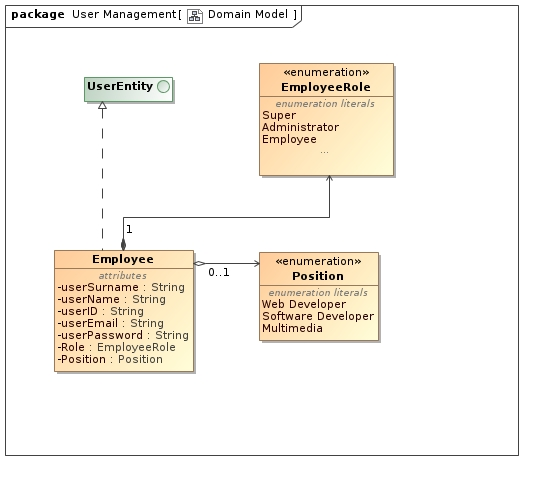
\includegraphics[scale=0.6]{../Images/User Domain Model.jpg}
		\caption{User Management Domain Model}
	\end{center}
\end{figure}

\pagebreak

\section{Integration and Pre-processing}
\subsection{Scope}
\begin{figure}[H]
	\begin{center}
		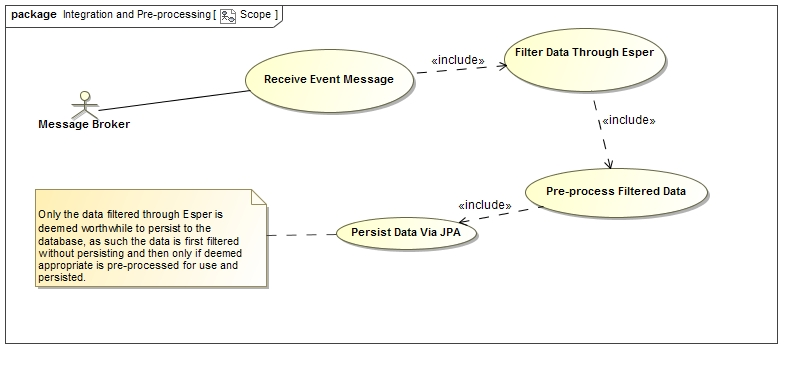
\includegraphics[scale=0.6]{../Images/Integration_Scope.jpg}
		\caption{Integration and Pre-processing Scope}
	\end{center}
\end{figure}
The scope of the integration module includes:
\begin{itemize}
	\item Events are received through RESTful services that are made available to event emitting system. There is no need for polling these systems.
	\item Each event is mapped to a JAVA POJO and is persisted. Along with being persisted each event object is also placed onto a message queue where a CEP Engine will act as the consumer on the other end.
	\item Algorithms are applied to the persisted data to generate reports.
\end{itemize}

\subsection{Domain Model}
\begin{figure}[H]
	\begin{center}
		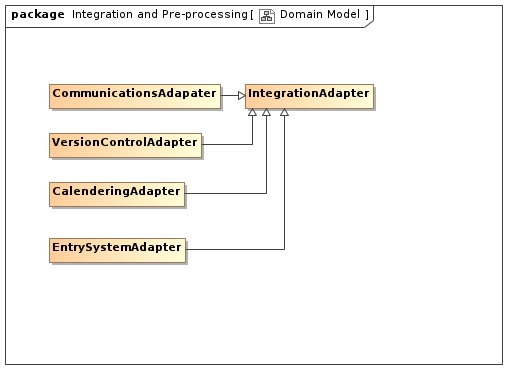
\includegraphics[scale=0.75]{../Images/Integration Domain Model.jpg}
		\caption{Integration and Pre-processing Domain Model}
	\end{center}
\end{figure}

\pagebreak

\section{Algorithms}

Algorithms are used in the calculation of performance scores. The entire Algorithms module is built using the Strategy design pattern. This allows for using different algorithms during runtime to calculate the scores. Since the Strategy design pattern is followed, new algorithms can easily be added with minimal code modification.

\subsection{Scope}
\begin{figure}[H]
	\begin{center}
		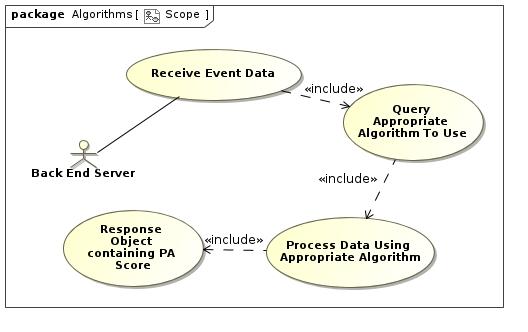
\includegraphics[width=\linewidth]{../Images/Algorithms Scope.jpg}
		\caption{Algorithms Scope}
	\end{center}
\end{figure}
The scope of the algorithms module includes:
\begin{itemize}
	\item Determining which statistical algorithm will be appropriate with regards to the employee. 
	
	\item Different algorithms can be applied to different types of employees.
	
	\item Applying this algorithm to the data provided, and then presenting employee performance scores accordingly.
\end{itemize}

\subsection{Domain Model}
\begin{figure}[H]
	\begin{center}
		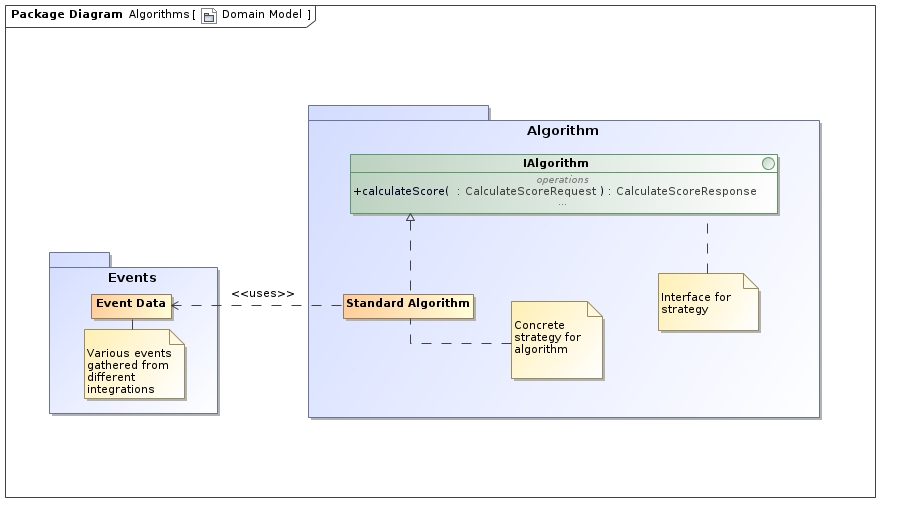
\includegraphics[width=\linewidth]{../Images/Algorithms_Domain_Model.jpg}
		\caption{Algorithms Domain Model}
	\end{center}
\end{figure}

\subsection{Service Contract}
\begin{figure}[H]
	\begin{center}
		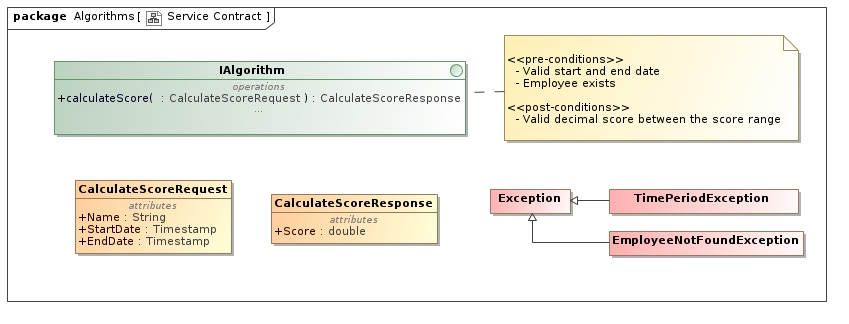
\includegraphics[width=\linewidth]{../Images/Algorithms_Service_Contract.jpg}
		\caption{Algorithms Service Contract}
	\end{center}
\end{figure}

\pagebreak

\section{Reporting}

The reporting component allows for the processing and generation of data. This data allows users to see their current performance. The reporting component allows for generation of three types of reports: summarised and detailed reports as well as generation of a performance score.

\subsection{Scope}
\begin{figure}[h!]
		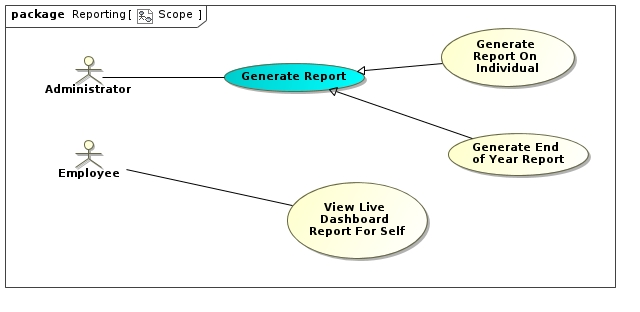
\includegraphics[width=\linewidth]{../Images/Reporting Scope.jpg}
		\caption{Reporting Scope}
		\centering
\end{figure}
The scope of the reporting module includes:
\begin{itemize}
	\item Administrators such as HR may request reports on individual employee's performance.
	\item All users, excluding administrators, may view their own dashboard which contains information regarding their current performance and personal details.
\end{itemize}

\subsection{Domain Model}
\begin{figure}[H]
	\begin{center}
		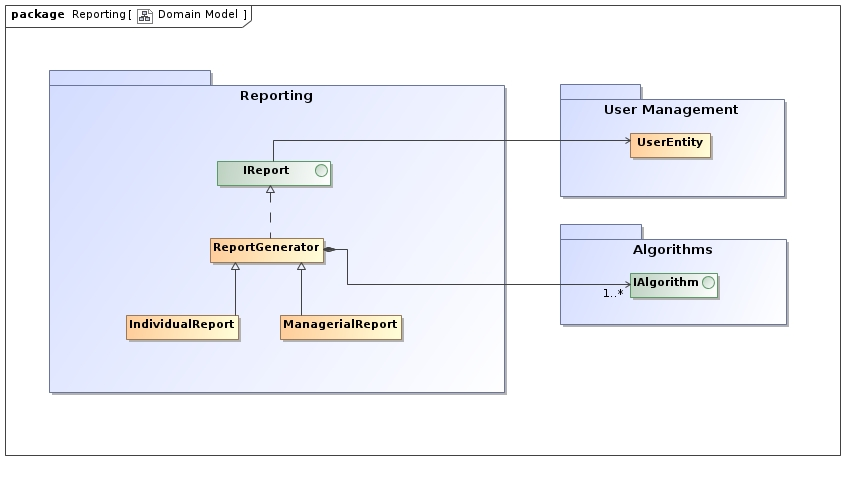
\includegraphics[scale=0.45]{../Images/Reporting Domain Model.jpg}
		\caption{Reporting Domain Model}
		\centering
	\end{center}
\end{figure}

\subsection{Service Contracts}
\begin{figure}[h!]
	\begin{center}
		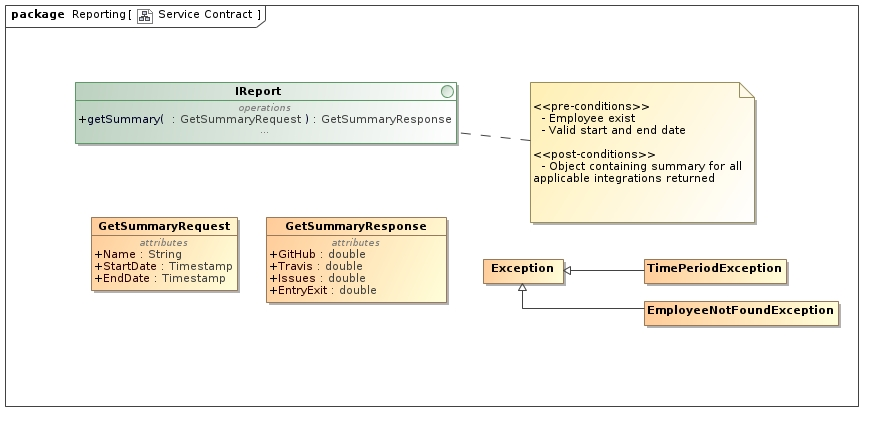
\includegraphics[width=\linewidth]{../Images/GetSummary Service Contract.jpg}
		\caption{Get Summary Service Contract}
	\end{center}
\end{figure}


\begin{figure}[H]
	\begin{center}
		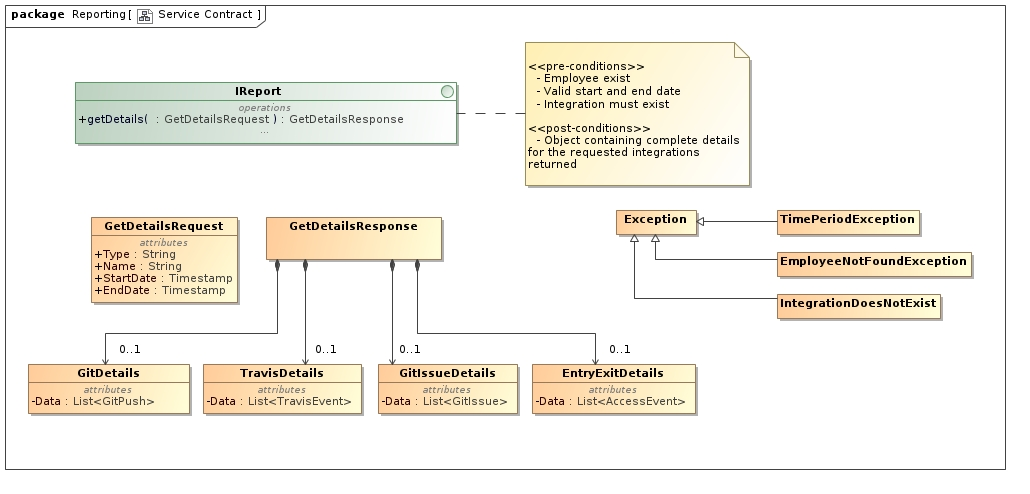
\includegraphics[width=\linewidth]{../Images/GetDetails Service Contract.jpg}
		\caption{Get Details Service Contract}
	\end{center}
\end{figure}


\begin{figure}[H]
	\begin{center}
		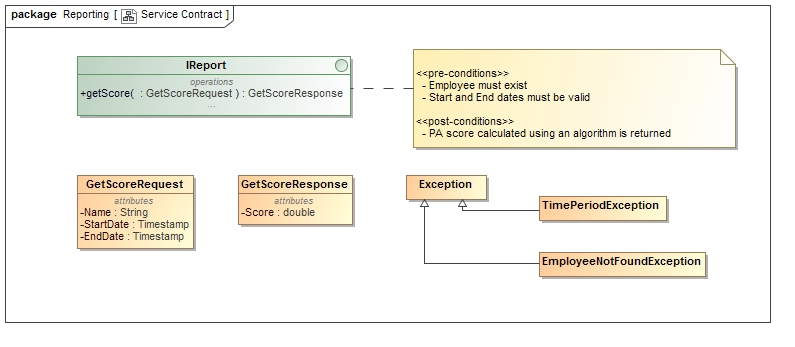
\includegraphics[width=\linewidth]{../Images/getScore Service Contract.jpg}
		\caption{Get Score Service Contract}
	\end{center}
\end{figure}


\pagebreak

\section{Notifications}
\subsection{Scope}
\begin{figure}[H]
	\begin{center}
		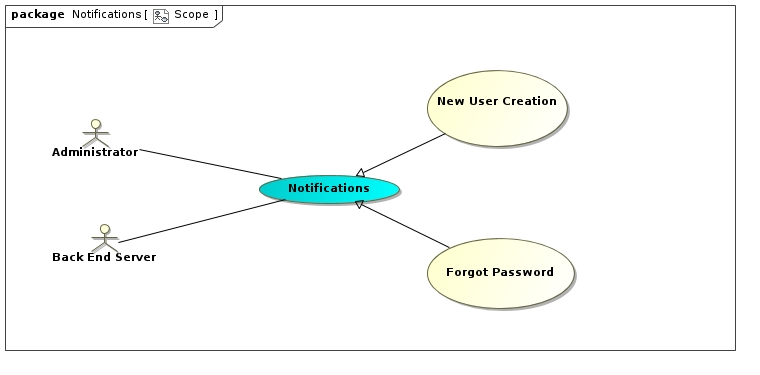
\includegraphics[width=\linewidth]{../Images/Notification Scope.jpg}
		\caption{Notifications Scope}
	\end{center}
\end{figure}
The scope of the notifications module includes:
\begin{itemize}
	\item When a new User is created by an Administrator, a notification will be sent to the user with initial passwords and information.
	\item When a user forgets their password, a temporary password will be sent to the user and more instructions to change their password.
\end{itemize}


\subsection{Domain Model}

\begin{figure}[H]
	\begin{center}
		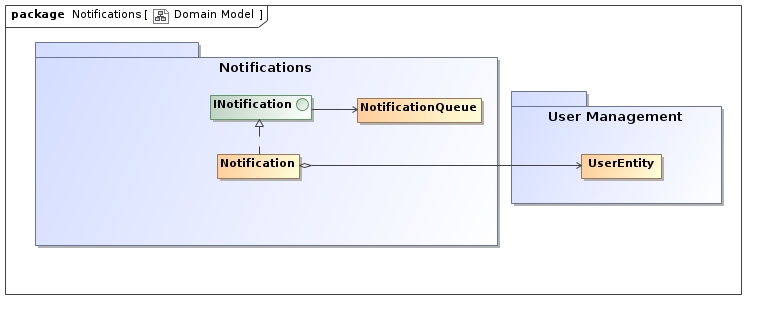
\includegraphics[width=\linewidth]{../Images/Notifications Domain Model.jpg}
		\caption{Notifications Domain Model}
	\end{center}
\end{figure}

\section{Forecasting}

The forecasting module is responsible for allowing the addition, modification and deletion of forecasted values. These values are predictions made by management which employees must try to conform to. Forecasted values may be used in conjunction with algorithms to allow for a more accurate calculation of performance scores. Forecasted values are contained in integrations. A manager is allowed to modify and add integrations along with forecast values.

\begin{itemize}
	\item To allow for pluggability the forecasting module consists of a contract. All realizations of the contract must adhere to the methods defined within the contract.
	
	\item Underlying representations of the forecasted values can be of any type and can be stored in any manner deemed beneficial.
	
	\item Since the forecasted values can have any representation, all necessary logic with regards to processing the data will be contained in the methods defined within the contract. This removes 'plumbing code' in the other components of the system.
	
	\item Since all forecast data processing occurs within the forecasting module only, it can be seen as a layer of abstraction over the representations of the forecasts themselves. The other components within the system will have no knowledge of the representation and will have controlled access to the data through the given contract.
	
	\item Representation of the forecast data can easily be changed without having to affecting the rest of the system. Forecast representations may be: JSON, XML, plain text etc. 
\end{itemize} 

\subsection{Service contracts}

\begin{figure}[h!]
	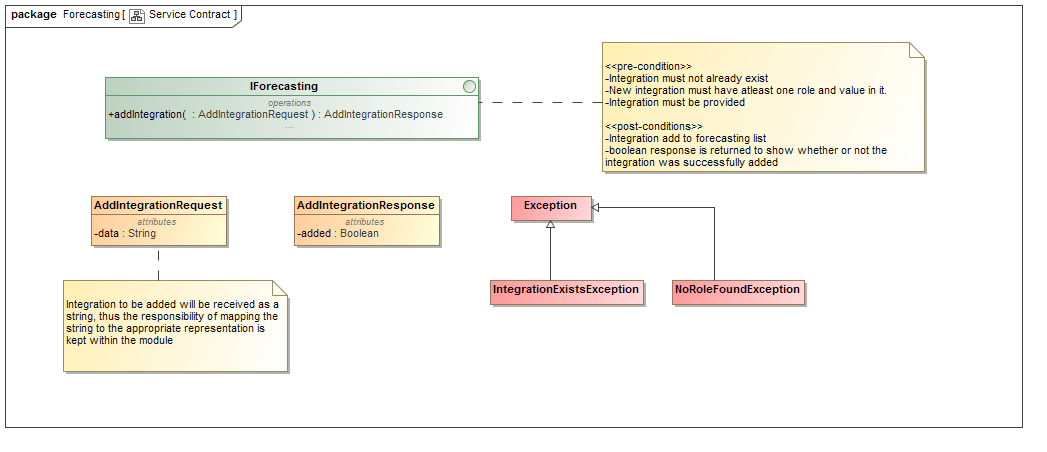
\includegraphics[width=\linewidth]{../Images/addIntegration_Service_Contract}
	\caption{Service contract for adding integrations}
\end{figure}

\begin{figure}[h!]
	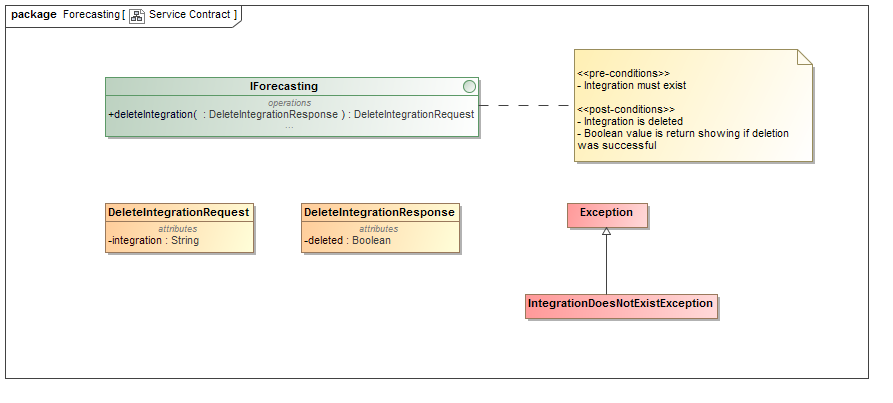
\includegraphics[width=\linewidth]{../Images/delete_integration_Service_Contract}
	\caption{Service contract for deleting integrations}
\end{figure}

\begin{figure}[H]
	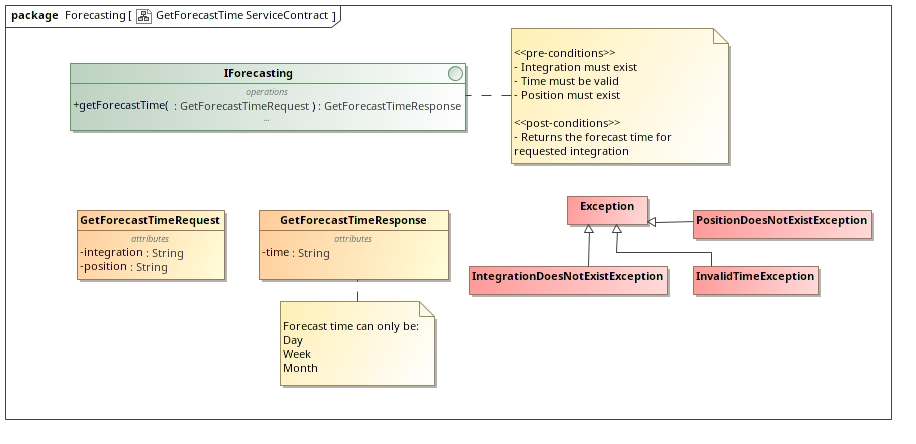
\includegraphics[width=\linewidth]{../Images/GetForecastTime ServiceContract}
	\caption{Service contract for getting a forecast timespan}
\end{figure}

\begin{figure}[H]
	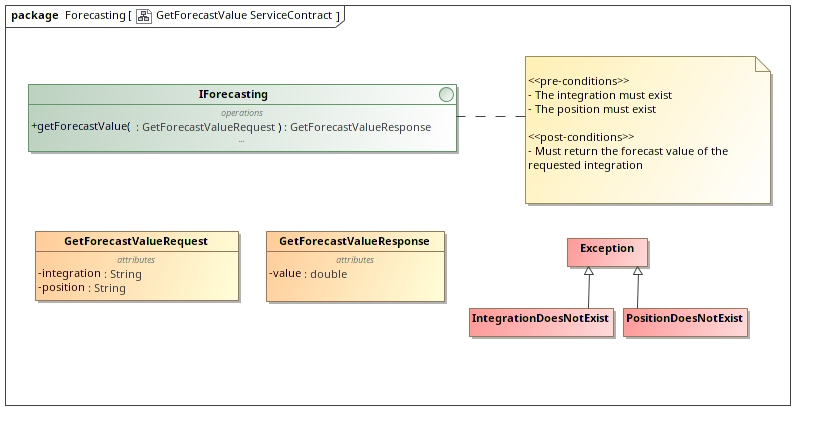
\includegraphics[width=\linewidth]{../Images/GetForecastValue ServiceContract}
	\caption{Service contract for getting a forecast value}
\end{figure}

\end{document}